\chapter{Implementation}
This chapter is concerned with the implementation details of the individidual components introduced in Chapter \ref{chapter:4}. This includes the development of the Unity application responsible for producing a video stream from the front-facing camera of the Hololens, the development of the human detection and direction system, as well as the reactive control systems implemented on ARTA. Previous work in the PRL had utilized the Hololens camera to capture images that were then processed on an external computer, but where this project differs is that a video stream was required to be able to perform real-time object detection. As such, a large amount of time was spent at the very beginning of the project trying to produce a video stream, since the whole project depended on this form of visual input.

\begin{figure}[ht]
	\centering
	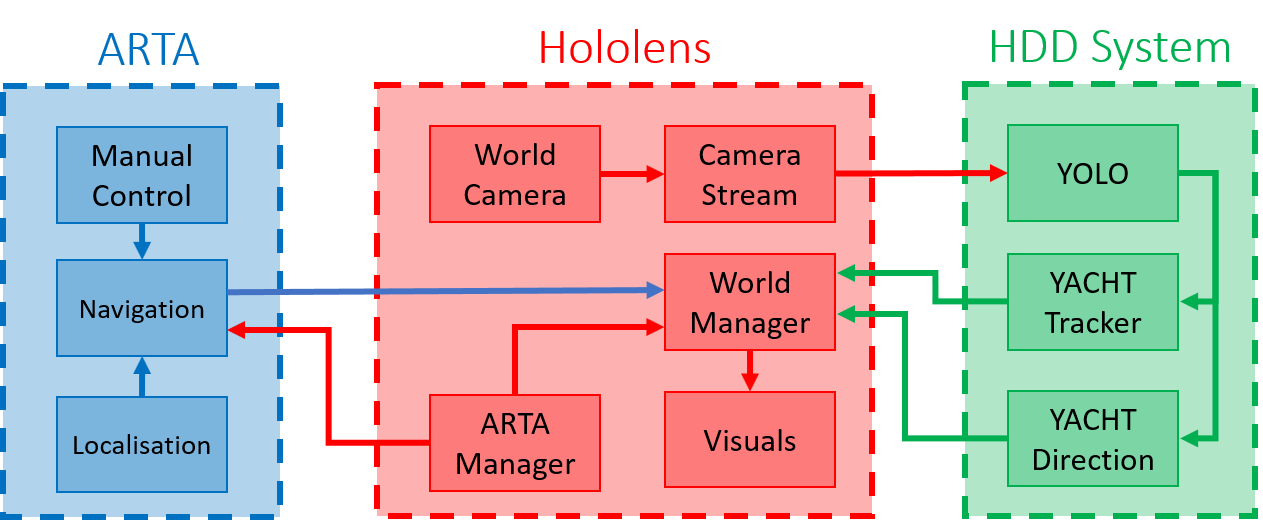
\includegraphics[width=1.0\linewidth]{img/chapter5_implementation/detailedSystemDiagram.png}
	\caption{System diagram detailing individual components}
	\label{fig:detailedHL}
\end{figure}

Figure \ref{fig:detailedHL} is a more detailed diagram of the high level system digram presented in Figure \ref{fig:simplifiedHL}. We show the communication between the three seperate devices, and how each node can be broken down into smaller nodes running specific computations. For the rest of this report, we represent ARTA, Hololens and HDD system components with the colours blue, red and green respectively.

%\section{Hololens Video Camera Stream}
%For this project to begin, it was absolutely essential to stream the front-facing camera on the Hololens to another PC. Once it had been proven that this was possible, work on the rest of the project could begin. As such, the first month of the project was spent comparing different camera streaming methods. As mentioned in Section \ref{sec:videoStreaming}, we briefly spent some time attempting to use the HoloLensForCV library from Microsoft. However, after speaking with several members of the PRL, it was decided the best method would be to use the Unity application approach as a base.


\section{Human Detection \& Direction System}
In order to be able to infer the direction people are walking in, it is necessary for the system to be able to detect humans. Only after detection is it possible to discern the motion of individuals, which can be achieved through object tracking and body pose estimation. This section is concerned with the implementation of the methods needed to perform the direction prediction, as well as how the system communicates between its nodes. Figure \ref{fig:detailedHDD} shows the breakdown of the HDD node into its seperate components. 

\begin{figure}[ht]
	\centering
	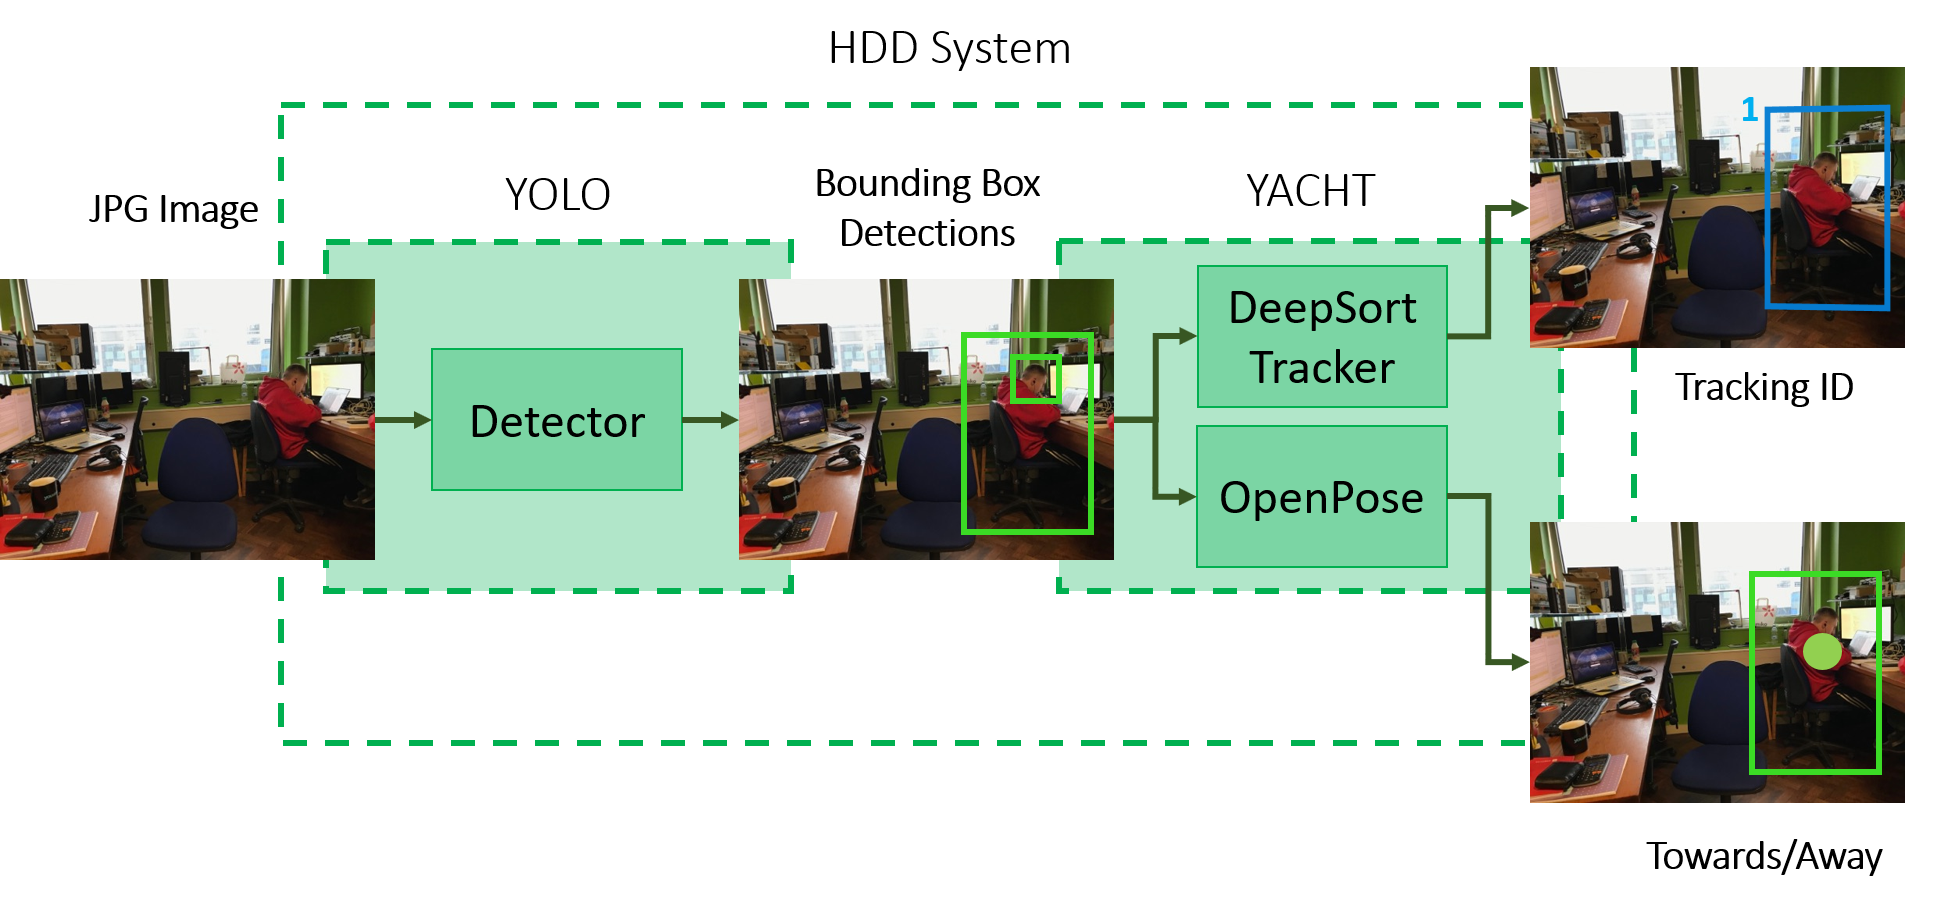
\includegraphics[width=1.0\linewidth]{img/chapter5_implementation/hddSystemDiagram.png}
	\caption{Individual nodes in HDD System}
	\label{fig:detailedHDD}
\end{figure}

We begin this section by listing the hardware requirements for the system. Due to the nature of the HDD, and its reliance on modern deep learning techniques, access to a modern GPU is essential. We refrain from trying to explain step-by-step how to setup the hardware and software, and instead point the reader in the direction of a Medium article\footnote{https://link.medium.com/xQ5w2FMXoX} which covers this topic.

\subsection{Hardware \& Software Dependencies}

\subsubsection{Hardware}
We implemented the HDD system on a desktop computer connected to the Imperial College network. Due to the real-time computer vision requirements of this project, the computer was chosen due to the GTX 1050Ti GPU with 4GB video RAM available on the system. The computer also had an Intel i7-2600 CPU and 8GB DDR3 RAM.

\subsubsection{Software}
We have refrained from posting every single Python dependency for the project. A complete listing is available in the appendix. The following software dependencies are required to run this project:
\begin{itemize}
	\item Ubuntu 16.04
	\item Python 2.7
	\item OpenCV 3.0
	\item ROS Kinetic
\end{itemize}

Due to the deep learning component of the project, the following software dependencies are essential:
\begin{itemize}
	\item Nvidia Graphics Drivers 
	\item CUDA 8.0 Toolkit
	\item cuDNN 6.0
	\item Darknet
	\item Tensorflow-GPU
	\item Caffe
\end{itemize}

\subsection{YOLO Object Detector}
As mentioned in Section \ref{sec:yolo}, we chose to use the YOLOv3-tiny architecture and trained it on the CrowdHuman dataset. We begin this section by introducing the reader to \textbf{Darknet}, the neural network framework YOLO is implemented on, and how we integrated it into ROS. We also briefly explain how the network detects objects, and compare YOLOv3-tiny with the more memory intensive YOLOv3. We then guide the reader through the training process, and the analysis we did to validate the human detection improvements compared to pre-trained models.

\subsubsection{Darknet}
Darknet\footnote{https://pjreddie.com/darknet/} is an open source neural network framework written in C and CUDA which supports both CPU and GPU computation \cite{darknet13}. The source code for the framework is freely available on Github, and can be used to train different neural network architectures in a manner similar to more conventional deep learning frameworks such as Tensorflow or Caffe.

\subsubsection{Darknet in ROS}
By definition, ROS is language-independent, although at the time of writing, three main libraries have been defined for ROS, making it possible to program ROS in Python, Lisp or C++. On the other hand, Darknet is implemented in C, due to the speed of compiled low-level languages in conjunction with CUDA. However, the Darknet framework is compiled into \textit{Shared Object (.so)} file, which is analogous to a Windows DLL. As such, it becomes possible to access the framework by writing wrappers around the compiled library file.

\paragraph{}Darknet has basic Python wrappers around the compiled library which convert Python datatypes into C and vice versa. However, the original wrappers for detection are written to run on images that are saved on disk. To integrate the framework into ROS, the node must be able to receive data from image topics with \code{CompressedImage} or raw \code{Image} messages.

\paragraph{}In Python, the JPG or PNG images received from the \code{CompressedImage} message can be converted to numpy arrays which store the RGB values. As such, we wrote Python wrappers for Darknet that would allow the framework to support images in the form of a numpy array as well as images saved on disk. This is done using the following code-snippet:

\begin{lstlisting}[language=Python]
# IMAGE: a C data structure used by Darknet
class IMAGE(Structure): 
	_fields_ = [("w", c_int),
				("h", c_int),
				("c", c_int),
				("data", POINTER(c_float))]
				
# Converts numpy array to Darknet IMAGE type
def nparray_to_image(img): 
	data = img.ctypes.data_as(POINTER(c_ubyte))
	image = ndarray_image(data, img.ctypes.shape, img.ctypes.strides)

	return image
\end{lstlisting}

We also wrote wrappers for the detection and return of the image bounding box co-ordinates which are used in the rest of the HDD system. The full code listing can be found in the appendix \footnote{https://github.com/alaksana96/darknet-crowdhuman}\footnote{https://github.com/alaksana96/fyp\_yolo}.

\subsubsection{YOLO algorithm}
The YOLO algorithm divides an input image into an $S\times S$ grid. Each grid cell can predict one object

\section{Hololens Unity Application}

\begin{figure}[ht]
	\centering
	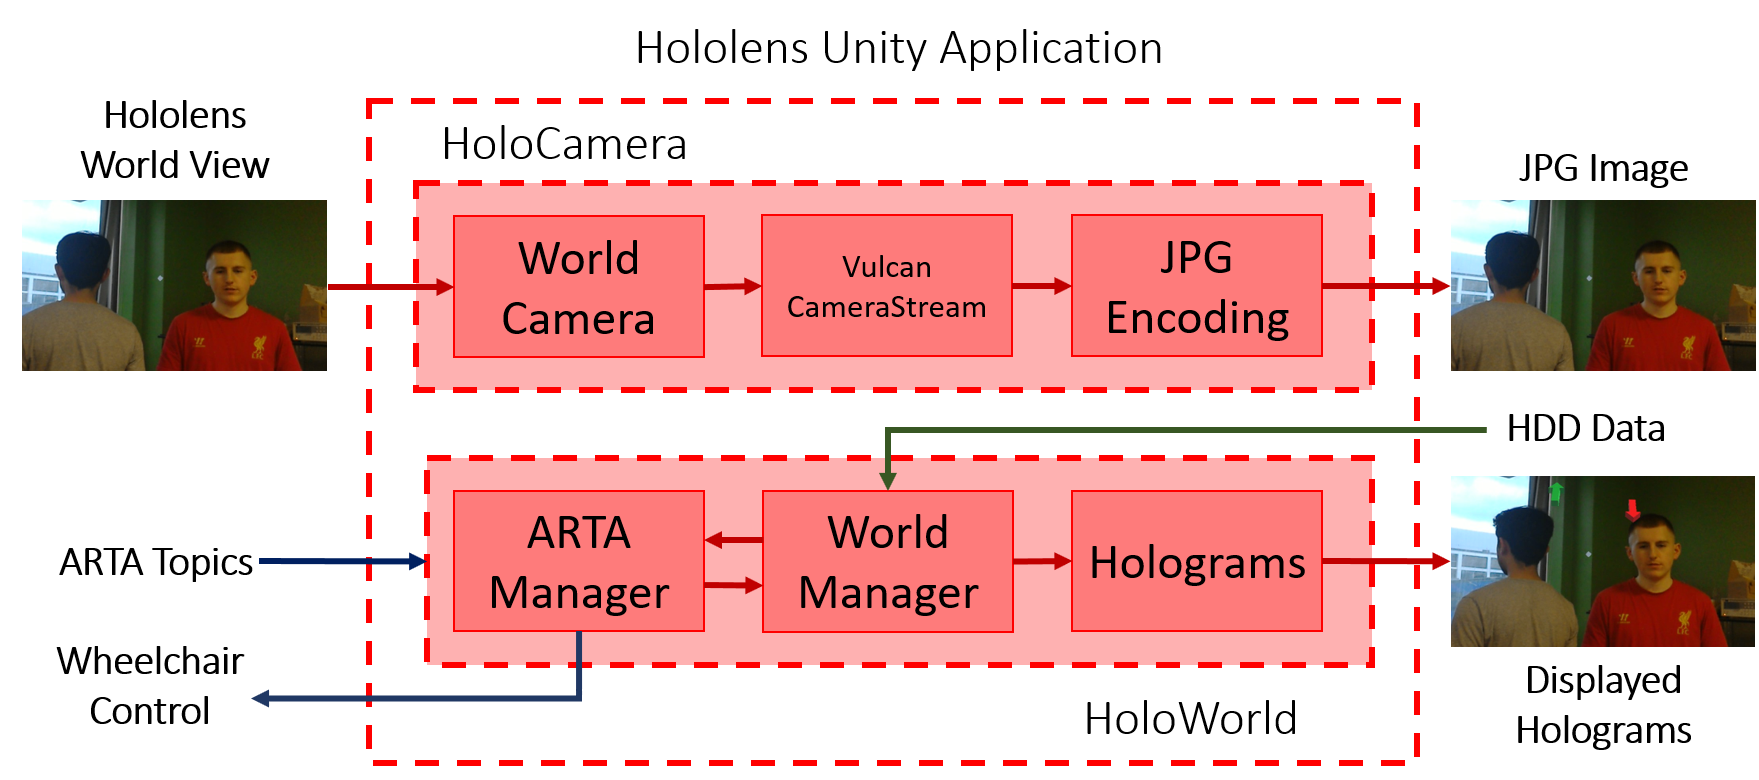
\includegraphics[width=0.85\linewidth]{img/chapter5_implementation/hololensSystemDiagram.png}
	\caption{Unity application running on the Hololens}
	\label{fig:detailedHololens}
\end{figure}
